\documentclass[12pt]{article}

%language
\usepackage[french]{babel}

% Set page size and margins
\usepackage[letterpaper,top=2cm,bottom=2cm,left=3cm,right=3cm,marginparwidth=1.75cm]{geometry}

% Useful packages
\usepackage{amsmath}
\usepackage{pdfpages}
\usepackage{graphicx}
\usepackage[colorlinks=true, allcolors=blue]{hyperref}
\graphicspath{ {./images/} }
\usepackage{amssymb}
\usepackage{ragged2e}
\usepackage{bm}
\title{\textbf{Équations de Maxwell}}
\author{Daniela D'Aliesio \\Bio Samir Gbian}


% Commands
\newcommand{\C}{\mathbb{C}}
\newcommand{\R}{\mathbb{R}}
\newcommand{\Q}{\mathbb{Q}}
\newcommand{\Z}{\mathbb{Z}}
\newcommand{\N}{\mathbb{N}}
\usepackage[parfill]{parskip}
\begin{document}

\begin{titlepage}
   \centering
    \vfill
    {\large UNIVERSITÉ DE MONTRÉAL\\DÉPARTEMENT DE MATHÉMATIQUES ET STATISTIQUE\par}
    \vspace{4cm}
    {\large LES ÉQUATIONS DE MAXWELL\par}
    \vspace{3cm}
    {\large PAR\\DANIELA D'ALIESIO ET BIO SAMIR GBIAN\par}
    \vspace{3cm}
    {\large FACULTÉ DES ARTS ET DES SCIENCES\par}
    \vspace{3cm}
    {\large TRAVAIL PRÉSENTÉ À JONATHAN GODIN\par}
    {\large DANS LE CADRE DU COURS MAT1410\par}
    {\large CALCUL 2\par}
    \vspace{2cm}
    {\large MAI 2023 \par}
\end{titlepage}

\section*{Introduction}
\justifying
\noindent Ce document mettra en lumière comment les théorèmes et les notions abordés dans le cours de Calcul 2 peuvent être appliqués et surtout, utilisés pour comprendre divers phénomènes en physique.

\noindent Au 19e siècle, le mathématicien James Clerk Maxwell introduit ses postulats portant sur des concepts d'électromagnétisme. Ces derniers devinrent des lois fondamentales en physique et plus tard, furent baptisés les équations de Maxwell. Plus spécifiquement, il s'agit de quatre équations couplées expliquant à la fois le comportement du champ électrique et du champ magnétique. Les voici ci-dessous : 

\begin {equation} \vec{\nabla} \bullet \vec{E} = \frac{\rho}{\varepsilon_0} \end{equation}
\begin{equation}\vec{\nabla} \bullet \vec{B} = 0\end{equation}
\begin{equation}\vec{\nabla} \times \vec{E} = - \frac{\partial \vec{B}}{\partial t} \end{equation}
\begin{equation}\vec{\nabla} \times \vec{B} = \mu_0\vec{j}+ \frac{1}{c^2}\frac{\partial \vec{E}}{\partial t}\end{equation}

\noindent Par la suite, ces équations menèrent à d’énorme progrès dans d’autres domaines de la physique (autre que l’électromagnétisme), car elles ont permis, notamment, de découvrir le concept d’onde électromagnétique, que la lumière en est une et également que la vitesse de la lumière est constante.


\noindent Avant de poursuivre et de mettre un cadre mathématique à l’électromagnétisme, voici un bref rappel de certains concepts fondamentaux.

\noindent \\\underline{Champ électrique :} Un champ électrique est un champ de vecteurs, noté $\vec{E}$, situé autour d'une particule chargée dans l'espace. Chaque vecteur possède un module qui est proportionnel à l'intensité de la force électrique générée par la charge. De plus, les vecteurs du champ électrique sont orientés dans la même direction que cette force. Plus spécifiquement, les lignes du champ électrique sortent des charges positives et se dirigent vers les charges négatives. 

\noindent \\\underline{Champ magnétique :} Un champ magnétique est aussi un champ vectoriel, mais est noté $\vec{B}$. Comme pour le champ électrique, le champ magnétique est proportionnel à l'intensité de la force magnétique et ses vecteurs sont orientés dans la même direction que cette force. Le champ magnétique peut être généré par des charges en mouvement, des courants électriques ou bien des aimants permanents. Lorsqu'il y a la présence d'un champ électrique et d'un champ magnétique, nous avons alors un champ électromagnétique. 

\newpage\section*{Légende}
\justifying
\noindent Spécifions maintenant les différents termes qui seront utilisés dans ce document:


\begin{center}
    champ électrique: $\vec{E}(\vec{r},t)$
    \\champ magnétique: $\vec{B}(\vec{r},t)$
    \\densité volumique de charges: $\rho_v(\vec{r},t)$
    \\courant électrique: $\vec{I}(\vec{r},t)$
    \\ densité de courant électrique: $\vec{J}(\vec{r},t)$ 
\end{center}


\noindent Notons que les équations de Maxwell expliquent le comportement des champs électriques et des champs magnétiques dans le cas de phénomènes électrodynamiques (Voir section plus bas). Par conséquent, chacune des fonctions introduites ci-haut dépendent du temps et de la position. Plus spécifiquement, dans ce document, nous parlerons de la position dans l'espace. Par exemple, soit un champ de vecteurs quelconque $\vec{v}$, alors nous noterons $\vec{v}:\mathbb{R}^3 \to \mathbb{R}^3.$ 

\noindent Cela signifie que $\vec{r}$, le vecteur position, sera également un vecteur tridimentionnel et selon le choix de coordonnées (cartésienne, cylindrique, sphérique) choisi, sera exprimé:
\begin{center}
    $\vec{r}(x,y,x)=r_x\hat{x}+r_y\hat{y}+r_z\hat{z}$
    \\$\vec{r}(\rho,\theta,z)= r_\rho \hat{\rho}+r_\theta \hat{\theta}+r_z \hat{z}$
    \\$\vec{r}(\rho,\theta,\phi)= r_\rho\hat{\rho}+r_\theta \hat{\theta}+r_\phi \hat{\phi}$
\end{center}
\noindent où   $\rho \in [0,\infty) ; \theta \in [0,\pi] ; \phi \in [0,2\pi]$

\noindent Le module du vecteur position représentera la distance entre deux points de l'espace, par exemple, la distance entre deux charges électriques.

\noindent Finalement, dans les équations de Maxwell, nous retrouvons également quelques constantes physiques telles que:
\begin{center}
    permittivité du vide: $\varepsilon_0$
   \\ perméabilité du vide: $\mu_0$
\end{center}
\noindent avec $\varepsilon_0, \mu_0 > 0$

\subsection*{Électrostatique VS Électrodynamique}
\noindent D'une part, l'électrostatique concerne les phénomènes électriques statiques, c'est-à-dire les charges électriques immobiles ou en équilibre ou encore possédant une vitesse négligeable. Cela permet de remarquer que le champ électrostatique est conservatif, car il ne varie pas avec le temps. D'autre part, l'électrodynamique traite des phénomènes électriques en mouvement et des interactions entre les charges électriques en mouvement et les champs électromagnétiques. Donc, le champ électrique en électrodynamique n'est pas conservatif, car celui-ci varie avec le temps.

\newpage\section*{Équation de Maxwell-Gauss}

Forme différentielle : $$\vec{\nabla} \bullet \vec{E} = \frac{\rho}{\varepsilon_0}$$\\

Forme intégrale : $$\iint_S \vec{E} \bullet d\vec{S} = \sum_i^n \frac{Q_i}{\varepsilon_0}$$\\

\noindent Cette première équation de Maxwell, nommée l'équation de Maxwell-Gauss, explique comment le flux du champ électrique est relié à la quantité de charges qui se retrouvent à l'intérieur d'un volume.

\noindent D'abord, écrivons la somme des charges intérieures comme: $$ \sum_i^n \frac{Q_i}{\varepsilon_0} = \frac{Q}{\varepsilon_0} $$ avec Q la charge totale.\\

\noindent Ensuite, par définition de la densité de masse volumique $\rho$, on a : $$\rho = \frac{Q}{V} \Rightarrow Q = \rho V.$$
\noindent En réécrivant le volume comme la somme infinie de volumes infinitésimaux, nous pouvons dire que:
$$V = \iiint_V \,dV$$ alors $$Q = \rho \iiint_V \,dV$$

\noindent En partant de la forme intégrale de l'équation de Maxwell-Gauss, nous avons alors: $$\iint_S \Vec{E} \bullet \,d\Vec{S} = \frac{Q}{\varepsilon_0} = \frac{\rho}{\varepsilon_0} \iiint_V \,dV = \iiint_V \frac{\rho}{\varepsilon_0} \,dV$$

\noindent Finalement, en appliquant le théorème de Gauss (également nommé le théorème de la divergence) que nous avons étudié dans le cours, nous savons que: 
 \[\iint_S{\vec{E}\bullet d\vec{S}}=\iiint_V{div\vec{E}dV}\]
\[\Rightarrow\iiint_V{\frac{\rho}{\varepsilon_0}dV=\iiint_V{div\vec{E}dV}}\]
\[\Rightarrow\frac{\rho}{\varepsilon_0}=div\vec{E}\]
\[\Rightarrow\frac{\rho}{\varepsilon_0}=\vec{\nabla}\bullet\vec{E}\]

\noindent Globalement, il faut retenir que le théorème de Gauss en physique est une version appliquée du théorème de la divergence.

\noindent \underline{Différence entre les pensées de Maxwell et de Gauss:} \\Gauss considérait uniquement les charges qui se retrouvent à l'intérieur de la surface sans considérer les charges qui se retrouvent à l'intérieur du matériau de la surface. Cependant, lorsque nous avons un champ électrique extérieur, celui-ci affectera, non seulement les charges à l'intérieur de la surface, mais également les charges à l'intérieur du matériau (ce que Gauss ne considérait pas). Maxwell a donc modifié l'équation de Gauss en prenant rho au lieu de $Q_i$ afin de prendre en compte les charges à l'intérieur du matériau également.


\newpage\section*{Équation de Maxwell-Thomson}

Forme différentielle : $$\vec{\nabla} \cdot \vec{B} = 0$$\\

Forme intégrale : $$\iint_S \vec{B} \bullet d\vec{S} = 0$$

\noindent La deuxième équation, nommée l'équation de Maxwell-Thomson, met en évidence que la divergence du champ magnétique, ou bien le flux du champ magnétique, à travers n'importe quelle surface fermée est toujours nul.

\noindent D'abord, nous remarquons que cette équation est très similaire à l'équation de Maxwell-Gauss (1) qui, elle, indique que la divergence du champ électrique n'est pas toujours nulle. Pourquoi cette différence? 

\noindent En effet, il peut exister, dans un espace quelconque, une particule unique qui est chargée, par exemple, un seul proton ou un seul électron. Dans ce cas, les lignes de champ électrique divergent dans l'espace et ne sont reliées à aucune autre source. Cependant, dans aucun cas n'existe-il un monopôle magnétique, car il y a toujours la présence de deux pôles (le pôle Nord et le pôle Sud). Par exemple, en brisant un aimant en deux, on obtient deux nouveaux aimants et non deux pôles séparés. Par conséquent, les lignes du champ magnétique qui sortent du pôle Sud annulent toujours ceux qui entrent par le pôle Nord. Donc, puisque le champ magnétique est à flux conservatif, sa divergence est toujours nulle. 

\noindent \underline{Explication théorique:}

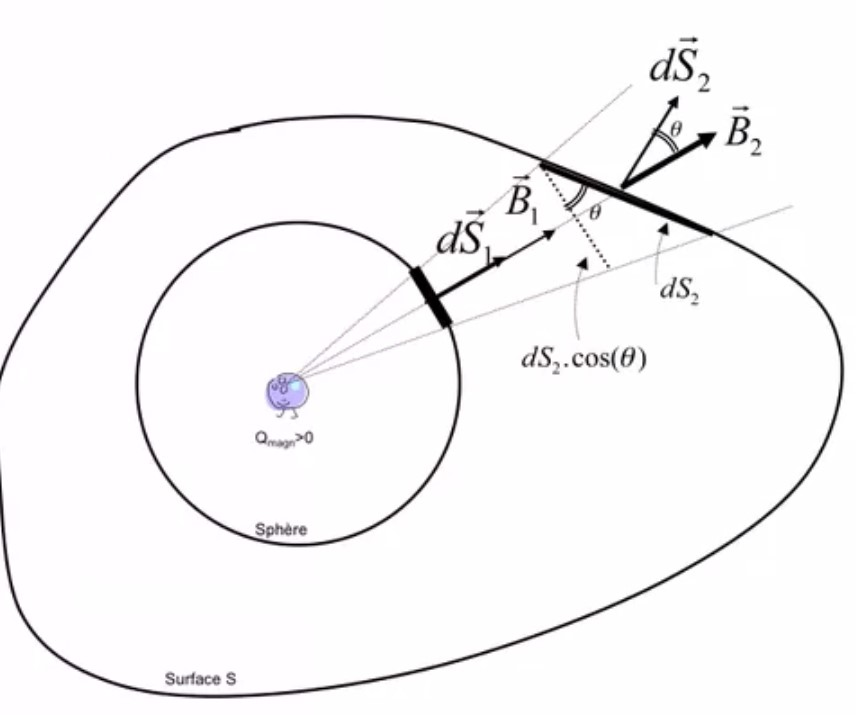
\includegraphics[scale=0.4]{Pictures/image.jpg}


\subsection*{1) Flux de B sur une sphère avec un monopôle magnétique}
\noindent Considérons une sphère et une charge magnétique ($Q_{magn}$) située au centre de cette sphère (nous savons que le monopôle magnétique n'existe pas dans la nature mais considérons le pour commencer l'exercice). Nous savons que $B = \frac{\mu_0 }{4\pi} \frac{Q_{magn}}{r^2}$. Nous avons : $$\phi(B) = \int_{Sph\Grave{e}re} \Vec{B} \bullet \,d\Vec{S} = \int_{Sph\Grave{e}re} B \bullet \,dS \bullet cos(B, dS) = \int_{Sph\Grave{e}re} B \bullet \,dS$$ $(\Vec{u} \cdot \Vec{v} = ||\Vec{u}|| \cdot ||\Vec{v}|| \cdot cos(\Vec{u}, \Vec{v})$).
\\ Ensuite, puisque $\vec{B}$ ne dépend que de la distance entre la charge magnétique et la surface de la sphère, son module sera donc constant sur toute la surface de la sphère (tous les point à la surface de la sphère sont équidistant du centre) et nous pourrons le sortir de l'intégrale. Nous obtenons ensuite :

\\ $$\phi = B \int_{Sph\Grave{e}re} \,dS = \frac{\mu_0 }{4\pi} \frac{Q_{magn}}{r^2} \cdot 4\pi r^2 = \mu_0 Q_{magn}$$.

\noindent Donc, le flux magnétique sur une spère avec un monopôle est $\mu_0 Q_{magn}$.

\subsection*{2) Flux de B sur une surface quelconque S avec un monopôle magnétique}
\noindent Plus nous nous éloignons de la charge, plus le module du champ magnétique diminue et plus la surface s'agrandit. Donc, il y a une certaine compensation entre la perte d'intensité et le gain en suface (voir image pour comprendre les symboles) :

$$\frac{B_2}{B_1} = \frac{\mu_0 }{4\pi} \frac{Q_{magn}}{r_2^2} \cdot \frac{4\pi }{\mu_0} \frac{r_1^2}{Q_{magn}} =  (\frac{r_1}{r_2})^2$$ 

\noindent Nous avons ensuite que :
$$\frac{B_2}{B_1} \frac{dS_2 cos\theta}{dS_1} = 1 \Rightarrow B_2 dS_2 cos\theta = B_1 dS_1$$ or, nous avons que 

$$B_2 dS_2 cos\theta = \Vec{B_2} \bullet d\vec{S_2}$$ et $$B_1 dS_1 = \Vec{B_1} \bullet \vec{dS_1}$$ donc, on a : $\Vec{B_2} \bullet d\vec{S_2} = \Vec{B_1} \bullet \vec{dS_1}$. Cela nous permet de remarquer que $$\int_{S} \Vec{B_1} \bullet \,d\Vec{S_1} = \int_{S} \Vec{B_2} \bullet \,d\Vec{S_2} = \mu_0 Q_{magn}$$

\subsection*{3) Flux de B sur une surface quelconque avec un dipôle magnétique}
\noindent Maintenant, puisque nous considérons un dipôle magnétique, nous avons $Q_+ = Q_{magn}$ et $Q_- = - Q_{magn}$. Nous obtenons :
$$ \int_{S} \Vec{B} \cdot \,d\Vec{S} = \int_{S} (\Vec{B}_{Q_+} + \Vec{B}_{Q_-}) \cdot \,d\Vec{S} = \int_{S} \Vec{B}_{Q_+} \cdot \,d\Vec{S} + \int_{S} \Vec{B}_{Q_-} \cdot \,d\Vec{S} = \mu_0 (Q_{magn} - Q_{magn}) = 0$$

\noindent Donc, par le théorème de Gauss, nous povons conclure :

$$\int_S \Vec{B} \bullet d\Vec{S} = \iiint_V \vec{\nabla} \bullet \Vec{B} \,dV = 0 \Rightarrow \vec{\nabla} \bullet \Vec{B} = 0$$.


\newpage\section*{Équation de Maxwell-Faraday}

Forme différentielle : $$ \vec{\nabla} \times \vec{E} = - \frac{\partial \vec{B}}{\partial t} $$

Forme intégrale : $$\oint_C \Vec{E} \cdot d\Vec{s} = -\frac{d}{dt} (\int_\Gamma \vec{B} \bullet d\Vec{S})$$

\noindent La troisième équation de Maxwell, nommée l'équation de Maxwell-Faraday, explique que la circulation du champ électrique autour d'une surface fermée est égale à la variation du flux magnétique à travers cette même surface.

\noindent \underline{Le champ électrique est-il toujours conservatif?}
\\\noindent Dans le cas d'électrostatique, le champ électrique est conservatif. Donc, par la proposition 2.3.14 vu dans le cours, nous savons que le rotationnel de $\vec{E}$, dans ce cas, est nul. 

\noindent De plus, par la définition 2.3.12 vu dans le cours, nous savons que comme le champ électrique est conservatif en électrostatique, il devrait exister un champ scalaire, disons f, tel que $E=\nabla f$. En effet, en physique, ce champ scalaire est nommé le potentiel électrique et est noté V. Le lien entre le champ électrique et son potentiel est alors que $\vec{E}=-\vec{\nabla}V$.

\noindent À partir de la notion du potentiel électrique V, il est ensuite simple de vérifier la proposition 2.3.14 comme ceci: $$\vec{\nabla} \times \vec{E}=\vec{\nabla} \times (-\vec{\nabla}V)=0$$

\noindent Cette égalité est toujours vraie en électrostatique, car le rotationnel d'un gradient est toujours nul.

\noindent Pour obtenir sa troisième équation, soit $\vec{\nabla} \times \vec{E}=-\frac{\partial \vec{B}}{\partial t}$, Maxwell a alors constaté que le champ électrique n'était non seulement composé d'un potentiel scalaire, mais également d'une autre composante...

\noindent \underline{À la recherche de la deuxième composante de $\vec{E}$:}
\\\noindent En effet, il existe un théorème mathématique, soit le théorème de Helmholtz-Hodge, qui dit: \textit{Soit $\vec{F}$, un champ vectoriel de classe $C^1 (D,\R^3)$ où $D$ est un domaine compact et connexe de frontière régulière, alors il existe un champ vectoriel $\vec{A}$ et un champ scalaire $\Psi$ définis sur D tels que $\vec{F}=\vec{rot}\vec{A}-\vec{\nabla}\Psi$.}

\noindent D'abord, comme nous avons mentionné précédemment, nous savons que $\vec{E}=-\vec{\nabla}V$. Par conséquent, posons comme hypothèse que le champ vectoriel $\vec{F}$ dans le théorème ci-haut est défini $\vec{F}=\vec{B}+\vec{E}$. Nous supposons alors que le champ magnétique est défini comme suit: \bm{ $\vec{B}=\vec{rot}\vec{A}$} avec $\vec{A}$, un potentiel vecteur.

\noindent Rappelons que l'objectif dans cette section est de trouver la deuxième composante de $\vec{E}$. Pour y parvenir, partons de la version intégrale de l'équation de Maxwell-Faraday:


\begin{align*}
\oint_C \Vec{E} \cdot d\Vec{s} &= \frac{d}{dt} (\int_\Gamma \vec{B} \bullet d\Vec{S})
\\\oint_C \Vec{E} \cdot d\Vec{s} &=-\frac{d}{dt}\iint_S \vec{B} \bullet \vec{n}d\vec{S}
\\\oint_C \Vec{E} \cdot d\Vec{s} &=-\iint_S-\frac{\partial}{\partial t} (\vec{B} )\bullet \vec{n}d\vec{S}
\\\oint_C \Vec{E} \cdot d\Vec{s} &=\iint_S-\frac{\partial}{\partial t} (\vec{rot}\vec{A})\bullet \vec{n}d\vec{S}
\\\oint_C \Vec{E} \cdot d\Vec{s} &=\iint_S\vec{rot}(-\frac{\partial \vec{A}}{\partial  t}) \bullet \vec{n}d\vec{S}
\end{align*}

\noindent Par le théorème de Stokes,
 $$ \oint_C \Vec{E} \cdot d\Vec{s} = \iint_S (\vec{rot}\vec{E}) \bullet \vec{n}d\vec{S} $$
\noindent Alors,
\begin{align*}
\iint_S (\vec{rot}\vec{E}) \bullet \vec{n}d\vec{S} & =\iint_S\vec{rot}(-\frac{\partial \vec{A}}{\partial  t}) \bullet \vec{n}d\vec{S}
\\\vec{E} & = -\frac{\partial \vec {A}}{\partial t}
\end{align*}
\noindent Nous avons obtenu la deuxième composante du champ électrique, donc:
$$\vec{E}=-\vec{grad}V-\frac{\partial \vec{A}}{\partial t}$$

\noindent À partir de cette nouvelle définition du champ électrique, nous pouvons maintenant obtenir la troisième équation de Maxwell.

\noindent \underline{Obtenir la troisième équation de Maxwell:}
\\\noindent Calculons le rotationnel du champ électrique:
\begin{align*}
\vec{rot}\vec{E}&=\vec{rot}(-\vec{grad}V-\frac{\partial\vec{A}}{\partial t})
\\\vec{rot}\vec{E}&=-\vec{rot}(\vec{grad}V)-\vec{rot}(\frac{\partial\vec{A}}{\partial t} )
\\\vec{rot}\vec{E}&=-\vec{rot}(\frac{\partial\vec{A}}{\partial t})
\\\vec{rot}\vec{E}&=-\frac{\partial}{\partial t}(\vec{rot}\vec{A}) \hspace{0.5em}(**)
\\\vec{rot}\vec{E}&=-\frac{\partial\vec{B}}{\partial t} \hspace{0.5em} car \vec{B}=\vec{rot}{\vec{A}}
\end{align*}

\noindent (**) Prouvons que $\vec{rot}(\frac{\partial\vec{A}}{\partial t})=\frac{\partial}{\partial t}(\vec{rot}\vec{A})$:

\noindent Soit un espace tridimentionnel, alors 


\noindent $\vec{rot}(\frac{\partial\vec{A}}{\partial t}) = \vec{\nabla} \times \frac{\partial\vec{A}}{\partial t}= $
$\begin{bmatrix}
    \frac{\partial}{\partial x} \\
    \frac{\partial}{\partial y} \\
    \frac{\partial}{\partial z}
\end{bmatrix}
\times 
\begin{bmatrix}
    \frac{\partial Ax}{\partial t} \\
    \frac{\partial Ay}{\partial t} \\ 
    \frac{\partial Az}{\partial t}
\end{bmatrix}$


\noindent $=(\frac{\partial}{\partial y}\frac{\partial Az}{\partial t}-\frac{\partial}{\partial z}\frac{\partial Ay}{\partial t})-(\frac{\partial}{\partial x}\frac{\partial Az}{\partial t}-\frac{\partial}{\partial z}\frac{\partial Ax}{\partial t})+(\frac{\partial}{\partial x}\frac{\partial Ay}{\partial t}-\frac{\partial}{\partial y}\frac{\partial Ax}{\partial t})$

\noindent $=\frac{\partial}{\partial t} (\frac{\partial Az}{\partial y}-\frac{\partial Ay}{\partial z})-\frac{\partial}{\partial t} (\frac{\partial Az}{\partial x}-\frac{\partial Ax}{\partial z})+\frac{\partial}{\partial t} (\frac{\partial Ay}{\partial x}-\frac{\partial Ax}{\partial y})$

\noindent $=\frac{\partial}{\partial t}(\vec{rot}\vec{A})$
\vspace{2em}
\\\noindent La notion de potentiel vecteur n'apparaît pas dans les cas d'électrostatique. En effet, comme il n'y a aucune dépendance du temps, $\vec{E}=-\vec{grad}V-\frac{\partial \vec{A}}{\partial t}$ devient tout simplement $\vec{E}=-\vec{grad}V$. Pour cette raison, c'est uniquement en régime stationnaire qu'il est possible d'affirmer que le champ électrique est conservatif.

\noindent \underline{Autre approche pour l'équation de Maxwell-Thomson:}
\\ \noindent Maintenant que nous avons la notion du potentiel vecteur, voici une approche beaucoup plus simple pour la deuxième équation: 

\newcommand{\proofend}{\hspace*{14cm} $\square$}

\noindent Par définition du potentiel vecteur magnétique $\vec{A}$, $\vec{B} = \vec{rot}\vec{A}$.\

\noindent Donc, nous avons que $div\vec{B} = div(\vec{rot}\vec{A}) = 0 \Leftrightarrow \vec{\nabla} \cdot \vec{B} = 0$.

\proofend


\newpage\section*{Équation de Maxwell-Ampère}

Forme différentielle :
$$\vec{\nabla} \times \vec{B} = \mu_0j + \frac{1}{c^2}\frac{\partial \vec{E}}{\partial t}$$

Forme intégrale : $$\oint_S \Vec{B} \bullet d\Vec{s} = \mu_0 (I + \frac{d}{dt} (\varepsilon_0 \int_\Gamma\Vec{E} \bullet d\Vec{S})) $$

\noindent La quatrième équation de Maxwell, nommée l'équation de Maxwell-Ampère, met en lumière l'interdépendance du champ électrique et magnétique. Plus spécifiquement, Maxwell découvre qu'un champ magnétique peut être engendré par la variation d'un champ électrique.

\noindent\underline{Loi d'Ampère:}
\\\noindent D'après le théorème d'Ampère, nous avons que $\vec{\nabla} \times \vec{B} = \mu_0\vec{\jmath}$, où $\vec{\jmath}$ représente la densité de courant électrique. Mais, cette relation n'est valide qu'en électrostatique.

\noindent En effet, il existe des lois en physique qui sont considérés comme étant plus fondamentales que les équations de Maxwell. C'est d'ailleurs en appliquant la loi d'Ampère au cas d'électrodynamique que cette dernière contradit une des lois fondamentales, soit celle de la conservation de la charge. 

\noindent Par définition de la densité du courant, nous savons que la densité de courant surfacique est égale à:
$$\vec{\jmath}=\frac{I}{S}$$
\noindent alors sur une surface orientable infinitésimale,
\begin{align*}
dI&=\vec{\jmath}dS
\\I&=\iint_S \vec{\jmath} \bullet d\vec{S}
\end{align*}
\noindent Par le théorème de Gauss (théorème 2.4.15), nous avons alors que le flux de la densité de courant électrique qui passe à travers une surface est égale à:
$$\iint_S \vec{\jmath} \bullet d\vec{S}=\iiint_V (\vec{\nabla}\bullet\vec{\jmath})dV$$

\noindent Par la suite, nous allons nous servir d'une équation mathématique nommée l'équation de continuité. Celle-ci explique que le flux d'une certaine quantité qui entre à travers une surface est égale au flux qui sort de cette même surface. Considérons d'abord $I=\iint_S \vec{\jmath} \bullet d\vec{S}$ comme le flux qui entre à travers une surface. Ensuite, par l'équation de continuité, nous savons que s'il y a des charges qui entrent, alors il y a également des charges qui sortent. Puisque le courant est défini comme la variation de charges électriques par rapport au temps, nous pouvons dire que la quantité qui sort est définie comme $I=-\frac{dQ}{dt}=-\frac{d}{dt}\iiint_V \rho dV$ (le signe moins vient du fait que le nombre de charges diminue en sortant du volume). 

\noindent Par l'équation de continuité, nous avons alors,
$$\iiint_V(\vec{\nabla}\bullet\vec{\jmath}) dV = -\frac{d}{dt}\iiint_V \rho dV = -\iiint_V \frac{\partial p}{\partial t} dV$$
$$\vec{\nabla} \bullet \vec{\jmath} = -\frac{\partial p}{\partial t}$$

\noindent En électrodynamique, comme il y a une dépendance du temps, l'égalité précédente est non nulle. $$\vec{\nabla} \bullet \vec{\jmath} = -\frac{\partial \rho}{\partial t} \ne 0$$ Cependant, que ce soit en électrostatique ou en électrodynamique, en calculant la divergence du théorème d'Ampère, nous avons: $$\vec{\nabla} \bullet \mu_o\vec{\jmath}=\vec{\nabla} \bullet (\vec{\nabla} \times \vec{B}) = 0$$

\noindent Puisque ceci contredit la loi fondamentale de la conservation de la charge, Maxwell a donc trouvé une façon de modifier le théorème d'Ampère.

\noindent\underline{Apport de Maxwell:}
\\Pour que le théorème d'Ampère soit valide en électrodynamique, il est nécessaire de rajouter un courant de déplacement noté $I_d$. Le courant de déplacement représente le taux de variation du champ électrique de déplacement ($\vec{E}_d$). De plus, on a que $\vec{E}_d = \varepsilon_0 \vec{E}$ et $\varepsilon_0$ représente la permittivité du milieu. 

\noindent Ensuite, par définition de la densité de courant électrique, nous savons que la densité surfacique correspond à $J = \frac{I}{S}$. Donc, on a :
$$\vec{J}_d = \frac{I_d}{S} \Rightarrow I_d = S\vec{J}_d$$ avec $J_d$ la densité du courant de déplacement. Ensuite, selon Maxwell, la densité de courant de déplacement correspond à la variation du champ électrique de déplacement par rapport au temps, c'est-à-dire: $$\vec{J}_d = \frac{\partial \vec{E}_d}{\partial t}$$ 

\noindent Ensuite, pour obtenir sa quatrième équation, Maxwell considéra le vecteur de densité de courant surfacique comme la surperposition de deux vecteurs, soient le vecteur de densité de courant trouvé par Ampère ($\vec{J}_A$) et également le vecteur de densité de courant de déplacement ($\vec{J}_D)$. Alors,
\begin{align*}
\vec{\nabla} \times \vec{B} &= \mu_0\vec{J}=\mu_0(\vec{J}_A+\vec{J}_D)
\\\vec{\nabla} \times \vec{B} &= \mu_0\vec{\jmath}+\mu_0\frac{\partial \vec{E}_D}{\partial t}
\\\vec{\nabla} \times \vec{B} &= \mu_0\vec{\jmath} + \mu_0\varepsilon_0\frac{\partial \vec{E}}{\partial t}
\end{align*}

\noindent Or, nous savons que la vitesse de la lumière $c = \frac{1}{\sqrt{\mu_0 \varepsilon_0}}$, alors: $$\vec{\nabla} \times \vec{B} = \mu_0\vec{\jmath} + \frac{1}{c^2} \frac{\partial \vec{E}}{\partial t}$$



%\newpage\section*{Référence}
%\begin{enumerate}
%    \item \href{file:///C:/Users/Samir/Desktop/Projet-Calcul2/Html%20file/Analyse%20vectorielle.html}{file}
%    \item \href{http://fiteoweb.unige.ch/~durrer/courses/eldynii.pdf}{Ruth Durrer - Courses}
%    \item \href{https://lesia.obspm.fr/perso/thierry-fouchet/optiqueI/chapitre1.pdf}{Lesia.obsm}
%    \item \href{https://opale.enim.univ-lorraine.fr/nowak2/electrotechnique_5KEL1M01/publications/5KEL1M01_web.publi/auroraW/co/flux_b_conservatif.html}{Vidéo %utilisée pour la deuxième équation}
%    \item \href{}{}
%    \item \href{}{}
%    \item \href{}{}
%    \item \href{}{}
%\end{enumerate}

\end{document}
